\section{Range Imaging}
\label{res:range imaging}

Intensity images such as MRI scans or heat maps applied to a scene based on a specific criteria related to the environment (such as temperature or humidity) do not impart much information about the surfaces they capture so estimating or inferring details from such images is limited. Range imaging encodes the positions of surface geometry directly so that the captured scene can be captured in terms of a depth map that can then be visualised. These images can be expressed in terms of a list of 3D coordinates in a frame or a sequence of frames with no strict ordering in the coordinate space. They can also be represented in terms of a matrix of depth values along the directions of the x,y image axes imposing a strict ordering on the points as a result \cite{Helmut2002}. Proper calibration of the equipment can yield distances in terms of standard metrics useful for calculating distances or heights in real time similar to the operation of LIDAR \cite{Maltamo2006}. 

%what each thing is and it's advantages/disadvantages

\subsection{Technologies}

Devices that produce range images can consist of a single camera, an array of cameras or a camera that is used in conjunction with a sensor array that is capable of capturing the depth information of a scene. Some of these technologies exploit the nature of the focal point or aperture in the device itself while others rely on the use of light both in the UV spectrum and outside of the visible plane.

\subsubsection{Stereo triangulation}

Stereo triangulation uses the concept of triangulation, determining a point in 3D space given it's projection onto $n$ images. Triangulation is achieved by identifying the camera projection function by which the 3D scene is projected onto 2D space. In the simplest case, this achieved using the camera's specific transformation matrix for achieveing this projection. By making this triangulation stereo, we are able to reconstruct a scene over the subset of points that the camera can capture. A simple triangulation method, $x \sim \tau(Y_1,Y_2,C_1,C_2)$, where $y_1$ and $y_2$ represent the homogeneous co-ordinates of the detected image points, $c_1$ and $c_2$ represent the camera transformation matrices gives $x$, the homogeneous representation of the 3D point. This method doesn't require specific illumniation conditions but requires that there is maximal correspondence for a given point captured by the cameras. This is made difficult due to the noise and geometric calibration inaccuracies that may result from a typical configuration \cite{Hausler1993}. \\

This method is also viable where a `plentopic camera' or single lens camera is used and reduces the overheads surrounding correspondence between image sensors in a binocular camera configuration. The use of this configuration was successfully used by Adelson in their replication of single lens stereo through the use of a plentopic camera \cite{Adelson1992}. They captured the structure of the optical light that hit the camera lens thus analysing the amount of light at each part of the scene allowing them to capture depth information from the virtual displacements achieved from their analysis of light hitting the optic lens. This particular method is only really suitable for achieving a depth map at a close range to the object rather than an entire scene due to the size of the lens aperture. Stereo triangulation remains widely used in the domain of robotic computer vision especially in the context of explorative robots that use SLAM (Simultaneous Localization and Mapping).

\subsubsection{Time-of-flight (TOF)}

Time of flight range imaging uses TOF cameras to capture a scene based on the notion of the known quantity of the speed of light. This is primarily done by measuring the speed at which light hits a particular point of a scene and then bounces back to the imaging sensor as a form of scannerless LIDAR, in this sense it is very similar to the operation of the Structured Light approach or the Microsoft Kinect but has the added algorithmic complexity which means that Time of flight camera's can also capture depth changes as they occur in real time, or relatively high resolution video frame rates (24fps) and it can be integrated into a configuration which allows for fast object capturing \cite{Cui2010}. Local rigid alignment between scans  is also possible using an Iterative Closest Point (ICP) algorithm. The passive nature in which Time-of-flight cameras capture scans is subject to a degree of noise and `Systematic bias'. This bias can lead to non-rigid scan distortions which affects the overall registration of the images captured by the camera. The distortions result from the 3D point measured by the depth camera being different from the orientation of the camera ray toward the point. TOF cameras are also expensive and require additional sensor arrays to operate accurately and effectively. 

\subsubsection{Coded Aperture}

Coded Aperture aims to retrieve raw depth information from a conventional RGB image captured using normal camera apparatus. This is achieved through measuring the colour intensity of the RGB image. The purpose of coded aperture is not to recreate a scene digitally nor achieve refined depth information for each point in the scene but to provide a cue for extended depth of field or markers for depth-based image editing. Levin et al in use a coded apeture to filter the image sensor so that the incident light on the camera lens is coded such that depth information can be extracted from the resultant image. The capturing of this depth map is useful where the focus or blur for a particular image is based on the referent of the depth map. It means that at the post processing stage, we can affect the image's focus using the depth map so different focus points can be yielded based on the information captured by the depth map. While this technique only works on still images and lacks the finer detail required by the 3D reconstruction of objects or an environment. 

\subsubsection{Structured Light}

This method uses a specific pattern of light which is ideally projected onto an object which is then captured by a camera or array of cameras. The most common pattern used is a series of strips projected onto a surface, the deformation and displacement of the projected light beams on the surface means that a typical configuration will be able to identify geometrics positions in 3D anywhere on the object after a sufficient number of captures have been taken as the structured light pattern converges to finer intervals. This structured light approach gives high accuracy stereo depth maps and in the majority of cases gives pixel-accurate correspondence between the subject captured the point registered in 3D space \cite{Scharstein2003}. The benefit of using stereo based depth maps is that the correspondences between the two images can be registered immediately without the requirement for further post processing. \\

Because of its accuracy and quality of the depth maps it produces, structured light mechanisms are frequently used in 3D Body Scanning configurations. Such a context yields accurate models of depth as their is only a single object of focus with which highly accurate displacement of light can be recorded. However, when applied to scenes with additional complexity containing a number of objects at different depths, Scharstein et al \cite{Scharstein2003} found that several small areas in a more complex scene shadowed under various types of strip illumination giving unknown disparities in the final depth map. Structured light is also poor for giving real time depth representation in fast moving scenes due to the low refresh rate inherent in the design of the algorithm.

\begin{figure}[ht]
\centering
        \begin{subfigure}(a)
            \label{lightscanner}
            \centering
            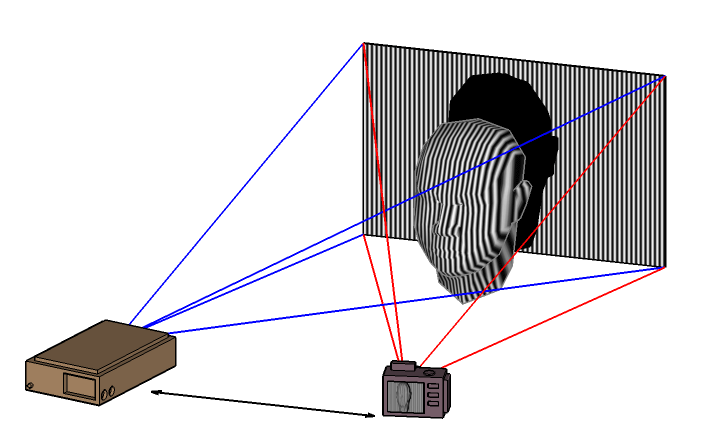
\includegraphics[scale=0.3]{images/structuredlightscanner.PNG}
            \end{subfigure}
            \begin{subfigure}(b)
                \label{shadowing}
                \centering
                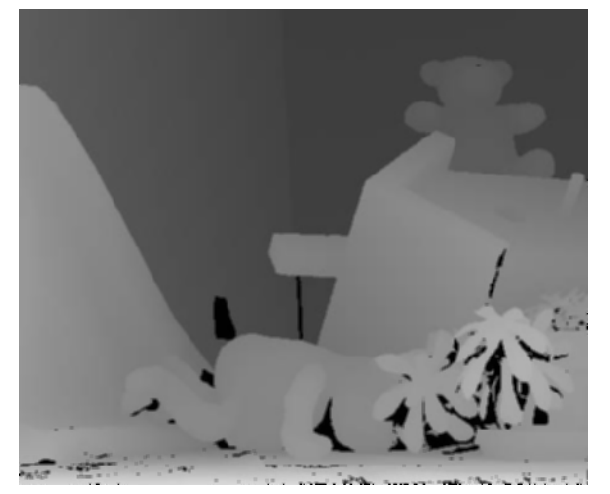
\includegraphics[scale=0.3]{images/occludedareas.PNG}
        \end{subfigure}
	    \caption{Typical structured light scanning configuration. Image on right shows shadowing in the depth map.}
\end{figure}

\subsubsection{The Kinect}

%include images, talk about the advantages/disadvantages of the device.

The hardware that The Kinect, originally a gaming device designed for the Xbox 360 gaming console, features is based on the principles of structured light as well as using aspects of stereo triangulation for the calculation and relative mapping of distances in a depth map. The Kinect projects a fixed pattern of infra-red dots onto a scene using an IR projector. Using a monochrome CMOS, the distance of each IR dot on the scene from the Kinect is captured and then post processed into a depth map. The benefit of having a fixed IR pattern means that the changes in the displacement of each of the fixed points can be recorded as subjects move in the scene. This allows for higher capture frame rate as the position in the x,y plane is maintained with only measurements in the z plane needing to be updated. This also means that calibration only needs to happen at the start of the capturing process or if the device is moved. \\ 

The Kinect also benefits from the use of the Kinect for Windows SDK \cite{SDK13}. The latest revision of the SDK (1.7 as of March 2013) includes support for the capturing and development of interactions such as those you would expect from a touch screen device. It also includes support for coarse spatio-temporal reconstruction of the scenes and objects that the camera captures using KinectFusion. The hardware as well as the inclusion of a stable established API provides accessible range imaging technology for developers and researchers, where traditional range imaging technology is out of reach due to the difficulty in achieving ideal scanning configurations or the overall initial cost. \\

\begin{figure}[ht]
\centering
        \begin{subfigure}
            \label{fig:kinectoffset}
            \centering
            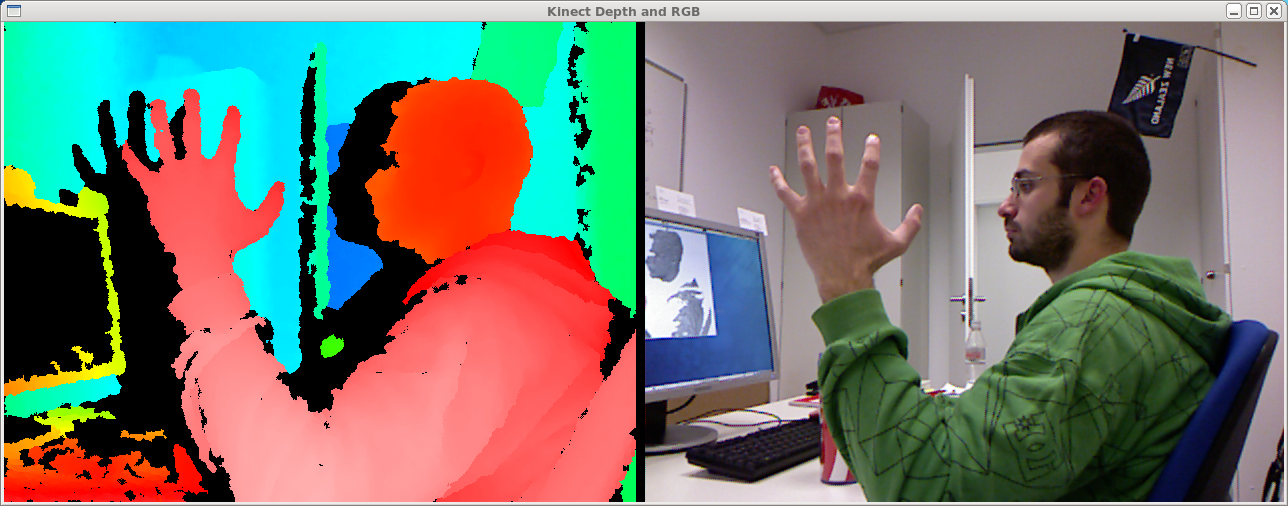
\includegraphics[scale=0.15]{images/kinectoffset.png}
            (a)
            \end{subfigure}
            \begin{subfigure}
                \label{kinectrecon}
                \centering
                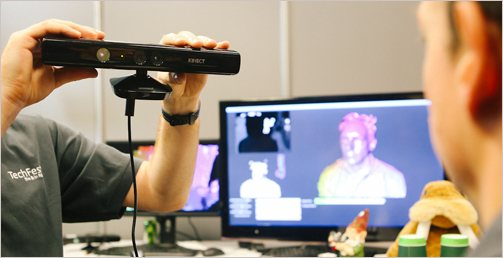
\includegraphics[scale=0.515]{images/kinectfusionrecon.jpg}
            (b)
        \end{subfigure}
        \caption{\emph{Top: }showing RGB and Depth Map with 10-20mm offset. \emph{Bottom: } non-rigid capture of human subject using Kinect SDK.}
\end{figure}

As observed in \ref{fig:kinectoffset}, the accuracy of the Kinect depth data is subject to the offset that exists between the RGB lens and IR receiver on the device. This offset manifests itself as an acute shadowing that forms due to the inaccurate orientation of the RGB camera with respect to the depth co-ordinate system. Further experimental results by Khoshelham's investigation \cite{Khoshelham2011} into the accuracy of depth data generated by the Kinect shows greater error registered the larger the distance due to the low resolution of depth data recorded at these distances \cite{Khoshelham2011}. The point clouds generated by the Kinect and that of a higher resolution laser based scanner recorded up to a  4cm discrepancy at larger distances. These point clouds were then subject to a registration exercise. The systematic error discovered in the point cloud pair generated by the Kinect demonstrated a greater error in plane registration compared to the laser based scanner. While the point density recorded by the Kinect was found to be lower than that of a laser scanner; a point cloud captured under ideal illumination conditions with sufficient calibration demonstrated only a small systematic error when compared to the laser based point cloud.

